\PassOptionsToPackage{table}{xcolor}
\documentclass[pdf]{beamer}
\mode<presentation>{\usetheme{Dresden}}
\usepackage{lmodern}
\usepackage[normalem]{ulem}
\usepackage{amsmath,textcomp,amssymb,geometry,graphicx,listings,array,color,amsthm}

\usepackage[noend]{algpseudocode}

\usepackage{tikz}
\usepackage{multicol}
\usetikzlibrary{shapes,snakes}
\usetikzlibrary{positioning}
\usetikzlibrary{arrows}
\usetikzlibrary{fit}
\usetikzlibrary{math}

%% For on-slide alerting of nodes
\tikzstyle{alert} = [text=black, fill=blue!20, draw=black]
\setbeamercolor{alerted text}{fg=blue}
\tikzset{alerton/.code args={<#1>}{%
  \only<#1>{\pgfkeysalso{alert}} % \pgfkeysalso doesn't change the path
}}

%% utils for removing uninteresting sections from the navbar
%% https://tex.stackexchange.com/questions/317774/hide-section-from-sidebar
\makeatletter
\let\beamer@writeslidentry@miniframeson=\beamer@writeslidentry%
\def\beamer@writeslidentry@miniframesoff{%
  \expandafter\beamer@ifempty\expandafter{\beamer@framestartpage}{}% does not happen normally
  {%else
    % removed \addtocontents commands
    \clearpage\beamer@notesactions%
  }
}
\newcommand*{\miniframeson}{\let\beamer@writeslidentry=\beamer@writeslidentry@miniframeson}
\newcommand*{\miniframesoff}{\let\beamer@writeslidentry=\beamer@writeslidentry@miniframesoff}
\makeatother

%% preamble
\title{Beating the House}
\subtitle{(You Will Not Beat the House)}
\author{A.C.}
\date{\today}

\AtBeginSection[]
{
  \miniframesoff
  \begin{frame}{Outline}
    \tableofcontents[currentsection,hideothersubsections]
  \end{frame}
  \miniframeson
}

\definecolor{darkred}{rgb}{0.7,0,0}
\definecolor{darkgreen}{rgb}{0,0.5,0}
\definecolor{darkblue}{rgb}{0,0,0.5}
\definecolor{darkpurple}{rgb}{0.4, 0.0, 0.4}

%% Code font settings
\lstset{
  showstringspaces=false,
  basicstyle=\scriptsize\ttfamily,
  commentstyle=\color{darkred},
  stringstyle=\color{darkgreen},
  keywordstyle=\bfseries\color{darkpurple},
}

%%%%%%%%%%%%%%%%%%%%%%%%%%
% Start of Actual slides %
%%%%%%%%%%%%%%%%%%%%%%%%%%
\begin{document}
\begin{frame}
  \titlepage
\end{frame}

\section{Putting It All On Black}

\subsection{Playing it Straight}

\begin{frame}{The Rules}
  \begin{enumerate}
  \item Place a bet with probability $p$ and payout ratio $r$.
  \pause\item The wheel spins.
  \pause\item Get paid \ldots or don't.
    \begin{enumerate}
      \item House advantage: $pr < 1$
    \end{enumerate}
  \end{enumerate}

  \[ X = \alpha \left(-1 + r\mathbb{I}(\text{Win})\right) \]
\end{frame}

\begin{frame}{Open Decisions}
  \begin{itemize}
  \item \sout{What bet to place.}
    \begin{itemize}
    \item Black feels lucky.
    \item $p \approx 0.47$
    \item $r = 2$
    \end{itemize}
  \pause\item How much to bet.
  \pause\item When to walk away.
  \end{itemize}
\end{frame}

\begin{frame}{The System}
  \begin{algorithmic}
    \Procedure{ConstantBets}{}
    \State $\alpha \gets 1$
    \While{\text{true}}
      \State $\text{bet}(\alpha)$
    \EndWhile
    \EndProcedure
  \end{algorithmic}
\end{frame}

\begin{frame}{Playing it Out}
  \[ W_n \sim \text{Bin(n, p)} \]
  \[ X_n = r \cdot W_n - n\]

  \pause
  \[ \text{Var}(X_n) = r^2 \text{Var}(W_n) = npqr^2\]
  \[ E(X_n) = r\cdot E(W_n) - n = npr - n = n(pr -1) \]
  \pause

  Expected losses grow as $n$, stddev as $\sqrt{n}$. Per Chebyshev, we
are going broke, \emph{almost certainly}.
\end{frame}

\subsection{Getting Back to Even}
\begin{frame}{The System}
  \begin{algorithmic}
    \Procedure{MartingaleBetting}{}
    \State $\alpha \gets 1$
    \While{\text{true}}
      \State $\text{bet}(\alpha)$
      \If{$\text{Win}$}
        \State \Return
      \Else
        \State $\alpha \gets 2 \cdot \alpha$
      \EndIf
    \EndWhile
    \EndProcedure
  \end{algorithmic}
\end{frame}

\begin{frame}{Playing it Out}
  Let $N$ be the round of betting where we finally win:

  \[ X_N = -1 - 2 - 4 \cdots -2^{N-1} + 2^N = \ldots \]

  \pause
  \[ = \alert{1} \]

  \pause

  $p$ nowhere to be found.\\

  \pause
  \alert{\emph{Guaranteed}} profit, on \alert{\emph{arbitrarily}} bad bets!
\end{frame}

\begin{frame}{Alas!}
  \begin{itemize}
  \item Very hard to get unlimited betting rounds.
    \begin{itemize}
    \item Credit limits
    \item Table limits
    \end{itemize}
  \end{itemize}

  \pause
  Exercise for the reader: what happens if we can be cut off before the payout?
\end{frame}

\subsection{Xeno's Gamble}
\begin{frame}{The System}
  \begin{algorithmic}
    \Procedure{AntiMartingaleBetting}{}
    \State $\text{target} \gets 2.0$
    \State $\text{reserves} \gets 1.0$
    \State $\alpha \gets 0.5$
    \While{$\text{reserves} < \text{target}$}
      \State $\text{reserves} \gets \text{reserves} + \text{bet}(\alpha)$
      \If{$\text{reserves} = \alpha$}
        \State $\alpha \gets 0.5 \cdot \alpha$
      \EndIf
      \If{$\alpha \leq 0.25 = \text{reserves}$}
        \State $\alpha \gets 2 \cdot \alpha$
      \EndIf
    \EndWhile
    \EndProcedure
  \end{algorithmic}
\end{frame}

\begin{frame}{Playing it Out}
  \[ P(\text{Lose}) = 0 \]

  \begin{center}
    Can't lose, must win\ldots Right?
  \end{center}
\end{frame}

\begin{frame}{Playing it Out II}
\begin{center}
  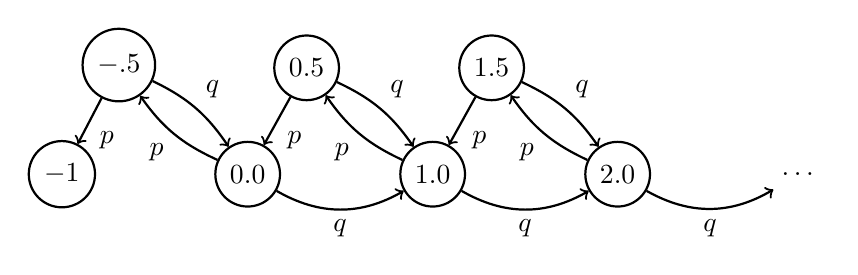
\begin{tikzpicture}[thick,auto,->]
    \node (Win)[alerton={<8>},circle, draw=black] {$-1$};
    \node[alerton={<1,6,9>}, circle, right = 1.5 of Win] (P0)[draw=black] {$0.0$};
    \node[alerton={<2,4,10>}, circle, right = 1.5 of P0] (P1)[draw=black] {$1.0$};
    \node[alerton={<11,13>}, circle, right = 1.5 of P1] (P2)[draw=black] {$2.0$};
    \node[alerton={<14>},circle, right = 1.5 of P2] (P3) {\ldots};
    \node[alerton={<7>}, circle, above left = 0.75 and 1 of P0] (PW5)[draw=black] {$-.5$};
    \node[alerton={<3,5>}, circle, above left = 0.75 and 1 of P1] (P05)[draw=black] {$0.5$};
    \node[alerton={<12>}, circle, above left = 0.75 and 1 of P2] (P15)[draw=black] {$1.5$};

    \path (PW5) edge node {$p$} (Win);
    \path (PW5) edge[bend left=15] node {$q$} (P0);
    \path (P0) edge[bend left=15] node {$p$} (PW5);
    \path (P0) edge[bend right] node[below] {$q$} (P1);

    \path (P05) edge node {$p$} (P0);
    \path (P05) edge[bend left=15] node {$q$} (P1);
    \path (P1) edge[bend left=15] node {$p$} (P05);
    \path (P1) edge[bend right] node[below] {$q$} (P2);

    \path (P15) edge node {$p$} (P1);
    \path (P15) edge[bend left=15] node {$q$} (P2);
    \path (P2) edge[bend left=15] node {$p$} (P15);
    \path (P2) edge[bend right] node[below] {$q$} (P3);
\end{tikzpicture}
\end{center}
\end{frame}

\begin{frame}{Playing it Out III}
\begin{align*} 
  P_{-1} &= 1\\
  P_{i} &= p^2 P_{i-1} + pqP_{i} + qP_{i+1}
\end{align*}
\pause
Let $\hat{p} = \frac{p^2}{1-pq}$, $\hat{q} = 1- \hat{p}$

\[P_i = \hat{p} P_{i-1} + \hat{q} P_{i+1}\]
\[\hat{p} P_i + \hat{q} P_i = \hat{p} P_{i-1} + \hat{q} P_{i+1}\]

  Massage. \pause series-term-cancellation. \pause limit as $n\rightarrow\infty$. \pause Massage.

\[ P_0 = \frac{\hat{p}}{\hat{q}}\]
\end{frame}


\begin{frame}{Alas!}
  We've created a gambler's ruin problem, just flipped and in log scale.

  \begin{itemize}
  \item Nonzero probability of winning \alert{\emph{at every step}}.
  \item Nonzero probability of \alert{\emph{never}} walking away from the table.
  \item Also, need to be able to place arbitrarily small bets.
  \end{itemize}

  \pause

  \[ p=0.48 \Rightarrow \frac{\hat{p}}{\hat{q}} \approx 0.44 \]

  \pause

  Would've been better off laying it all on black.
\end{frame}

\section{Fast Horses, Faster Money}
\subsection{}
\begin{frame}{The Rules}
  \begin{enumerate}
  \item $n$ horses running, each with probability of winning $p_i$ and payout odds $r_i$
    \begin{enumerate}
      \item House advantage: $\sum_i \frac{1}{r_i} > 1$
    \end{enumerate}
  \pause\item Bet $\alpha_i$ units on each horse
  \pause\item The horses run.
  \pause\item Get paid according to your wager on the winning horse.
  \end{enumerate}

  \[ X = \sum_i \left[ \alpha_i (-1 + r_i\mathbb{I}(h_i)) \right] \]
\end{frame}

\begin{frame}{Open Decisions}
  \begin{itemize}
  \item Which horse(s) to back.
  \pause\item How much to bet.
  \pause\item \sout{When to walk away.}
    \begin{itemize}
      \item We're going to do single round betting here.
    \end{itemize}
  \end{itemize}
\end{frame}

\begin{frame}{Pick the Right Horse}
  \begin{itemize}
  \item We could play it straight, as we did in roulette.
  \pause\item More (any) epistemic uncertainty
  \pause\item Might even be able to turn a profit, if you're smarter than the market.
  \pause\item Still gambling though.
  \end{itemize}
\end{frame}


\subsection{Some Low-Level Accounting}
\begin{frame}{The Booky's Favorite}
  \begin{itemize}
  \item Suppose there is an old nag in the race, Rocinante.
  \pause\item Rocinante is a long, long, \emph{long} shot. Maybe 1 in 1000.
  \pause\item Book-maker offers a special on Rocinante bets: 2000 to 1.
    \begin{itemize}
    \item Does not update the rest of the book.
    \item House advantage slips. Now $\sum_i \frac{1}{r_i} < 1$
    \end{itemize}
  \end{itemize}
\end{frame}

\begin{frame}{The Obvious Approach}
  \begin{itemize}
  \item Could just take the bookie up on the special.
  \pause\item Bet is positive valued in expectation
  \pause\item But I still need to make the rent this month, and this is a single round of gambling
  \pause\item Too rich for my blood, and it's still gambling.
  \end{itemize}
\end{frame}

\begin{frame}{Amongst the Tulips}
  \[ X = \sum_i \left[ \alpha_i (-1 + r_i\mathbb{I}(h_i)) \right] \]

  What happens if we try to clear $r_i$ out of our RV? \pause Set $\alpha_i = \frac{1}{r_i}$:

  \[ X = \sum_i \left( -\frac{1}{r_i} + \mathbb{I}(h_i) \right) = 1 - \sum \frac{1}{r_i}\]

  \pause

  That's a fixed payout.\\

  \pause

  A fixed, \alert{\emph{positive}} payout. This is what's known as a Dutch Book.
\end{frame}

\begin{frame}{Alas!}
  Finding a bookie setting a line that is susceptible to a Dutch Book is\ldots
  not easy.
\end{frame}

\subsection{A Bigger, Dutcher Book}
\begin{frame}{$N$ bookies, One Race}
  \begin{itemize}
  \item Suppose multiple bookies are taking action on a single race.
  \pause\item They have different clientelle, and are setting different lines
    \begin{itemize}
    \item Bookie doesn't care about odds, bookie wants to take a vig off of evenly spread bets.
    \item Just like we did with our Dutch book.
    \end{itemize}
  \pause\item Call the most favorable odds across all book makers for each horse $r^*_i$
  \end{itemize}
  \pause
  If $ \sum_i r_i^* < 1 $ we have a composite Dutch book! Let the arbitrage
times roll.
\end{frame}

\begin{frame}{Alas?}

  \begin{itemize}
  \item Efficient market theory is wrong.
    \begin{itemize}
    \item Not often wrong enough for this, though.
    \end{itemize}
  \pause\item With the right combination of speed and luck, however, arbitrage is possible.
  \begin{itemize}
  \item A frightening amount of effort goes into exactly this sort of game
  \item Usually against financial markets, though
  \end{itemize}
  \end{itemize}
  
\pause

Also, if we pull this off we haven't so much beaten the house as become it.

\end{frame}

\end{document}
